\documentclass[a4paper,12pt]{article}

\usepackage[utf8]{inputenc}
\usepackage[english]{babel}
\usepackage[margin = 1in]{geometry}
\usepackage{amsmath,amsthm,amssymb}
\usepackage{xcolor,graphicx}
\usepackage{hyperref}
\hypersetup{
    colorlinks = true,
    linkcolor = blue,
    citecolor = red,
    urlcolor = blue
}
\usepackage{booktabs}


\newcommand{\ind}[1]{\boldsymbol{1}\left\{ #1 \right\}}
\newcommand{\R}{\mathcal{R}}



\begin{document}

\begin{titlepage}
    \begin{center}
        \vspace*{1cm}
 
        \Huge{\textbf{Censored Data Analysis of\\ Tea Auction Pricing}}
         \vspace{1.5cm}
 
        \Large{\textbf{Subhrajyoty Roy\\Roll: MB1911}}
 
        \vspace{1cm}
        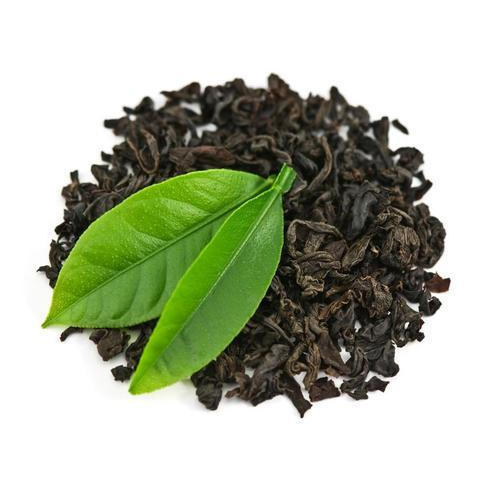
\includegraphics[width = 0.8\textwidth]{tealeaf.jpg}

        \vfill
             
        \normalsize{A report presented in partial satisfaction of the course ``Survival Analysis''\\
        as a part of ``Master of Statistics (M. Stat.) Programme''}
             
        \vspace{0.8cm}
                  
        Indian Statistical Institute, Kolkata\\
        \today             
    \end{center}
 \end{titlepage}


\section{Introduction}
Tea (Camellia sinensis) is a manufactured drink that is consumed across the world. Since the tea crop has specific tropical agro-climatic requirements, it is mostly produced in China, India, Sri Lanka, Vietnam etc., the Asian countries. The tea industry is one of the oldest organized industries in India with a large network of tea producers, retailers, distributors, auctioneers, exporters and packers. It provides a vital role in the Indian economy by being one of the major foreign exchange earners~\cite{sivanesan2013tea}. 

Tea is heterogeneous with a wide range of variety being produced throughout India. Almost $88\%$ of the tea produced in India are of CTC (Cut, Tear and Curl) type (the black tea leaf), with about $10\%$ being of an orthodox variety, and rest $2\%$ are green tea~\cite{arya2013indian}. CTC tea is largely graded as Broken Leaf, Dust and Fannings. Each of these grades has a dozen sub-grades based on the size of the grain etc. Several factors
influence the demand for tea, including the price and income variables, demographics, cultural background. Apart from consumption, other main drivers of international tea prices are trends and changes in per capita consumption, market access, the potential effects of pests and diseases on production, and changing dynamics between retailers, wholesalers and multinationals. To regulate this volatility in tea pricing, it is generally sold to the retailers through some regulatory e-Auction houses, which acts as an intermediary between the tea producers and the retailers.

\subsection{e-Auction and its relation to censoring}
Starting from the tea leaves produced in the tea gardens of Assam or Darjeeling (the major tea producers in India) to a beverage lying in our cup, there are many steps that it must go through. The tea leaves handpicked by the labours working in the garden is first moved to the tea factory associated with the garden, where the leaves are cut, torn and dried for several weeks, and then curled into tea dust which is packaged. Then, these packages are sent to auction houses, where these packages are opened and samples are collected. These tea samples are brewed and several experienced tea tasters taste them, and assigns some quality ranking, which is then transferred into a basic valuation for the corresponding packet. These samples are sent to some of the potential bidders as well. Finally, on the day of the auction, the packages are again sealed and are put for the auction where the retailers can bid~\cite{eauction-annexture}. These retailers, upon winning the auction bids, procure these tea packets from the auction houses and sells them in the market to consumers like us.

The censoring mechanism in the bidding comes from the peculiar setup of the second price closed bidding auction system. In the auction, the auction house poses an initial valuation of the tea packets based on the subjective judgement of its quality obtained from the appointed tea tasters. Since, tea is a perishable good, to increase the sell-ability of the packet, bidders are allowed to bid less than the initial valuation. As long as the final bid remains less than the initial valuation, the highest bidder needs to pay equal to his bid amount to the auction house. However, if the final bid exceeds the initial valuation, the highest bidder only needs to pay the amount equal to the second-highest bid. Therefore, the price which is recorded by the auction houses is either an uncensored observation of buyers' own valuation, or a censored observation of the buyer's own valuation censored by the second-highest bid. Let, $V_1, V_2, \dots V_n$ be the initial valuations for $n$ packets declared by the auction house, and let $P_1, \dots P_n$ be the selling price, then the observations are $(P_i, \delta_i)$, where 

\begin{equation}
\delta_i = \begin{cases}
    1 & \text{ if } V_i \geq P_i\\
    0 & \text{ if } V_i < P_i
\end{cases}; \qquad \text{ for } i =1, 2, \dots n,
\label{eqn:delta-i}
\end{equation}


\noindent denoting whether the underlying variable (i.e. the own valuation of the bidders, which is an indicator of the ultimate selling price to the consumers) is uncensored or not. 

\subsection{Existing Works}

Classical analysis of auction theory viewed auction as a game between the buyers and sellers where some incomplete information is provided through different bidding structures. Vijay krishna~\cite{krishna2009auction} has provided detailed mathematical treatment of various auction mechanisms such as sealed envelope auction, first and second-price auction, European, English and Dutch auction etc from a game-theoretic point of view where the payoff functions are explicitly known. Compared to this, viewing the selling price as a censored data in the context of auction theory is fairly new in practice. In many real-life scenarios, the payoff function is not known apriori, hence one must estimate these payoffs based on the censored bidding history available. George and Hui~\cite{george2012optimal}, provide an ingenious way to estimate demand in the auction market, under the Independent Private value model second-price auctions. The Private value model assumes that each of the signals about the actual price of the item to each of the bidders is independent. However, in most of the cases, the bidders are well-informed, hence their respective signals have a dependency, hence an independent private value model assumption is not justified.

Other than demand estimation, censored data on bidding history can prove useful in analyzing optimal bid for the bidders as well. In the online advertising industry, different companies bid for screen spaces of websites to show their advertisements, and a prediction about the winning price in the bid helps the bidders to secure screen spaces optimally~\cite{wu2015predicting}.


\subsection{Objective of the study}\label{sec:goal}

In the context of the tea auction of India, analysis shows that the auctioneer's valuation, which should have been only a measure of the quality of the item, becomes a causal variable for the demand signal of the bidders~\cite{dalal2020information}. Such an indication of causality and influence of the base price is also available in the context of tea auction in Kenya, Mombasa etc.~\cite{graham2019digital}, so the authorities have decided to hold offline auctions (where the bidders get to test the tea packets themselves) rather than ``e-Auction" held in online mode. One of the primary objectives of the study is to establish whether auction house provided valuation plays a significant role in the determination of the valuation of the bidders in the market. 

Also, since the auction house provided valuations are subjective and depend on the preferences and experiences of tea tasters, several bidders find it uninteresting to stay in the industry. Similar problems were also apparent in Coal block auctions till 2015~\cite{hariani2018auction}, which led the authorities to find a suitable substitute index number. This serves as a representative of its quality and well correlated with the bidder's proposed valuation, but remains free of any kind of subjective evaluation. The secondary goal is to provide a way to obtain such an index of quality for different types of tea.


\section{Description of the dataset}

We use the data\footnote{The data is not publicly available. Hence, is not used before except this work~\cite{dalal2020information}.} on e-Auction statistics of Kolkata dust tea provided by J. Thomas \& Co. Pvt. Ltd, which is the largest auctioneer in the world, handling over 200 million kg of tea a year, about one-third of all tea auctioned in India~\cite{dalal2020information}. The dataset contains e-Auction statistics from 2018 January to 2019 March. The bidding happens once a week, hence information about the packages displayed for bidding for that week is available, whether that package was sold or not. Apart from identification information on the tea package, the origin of the tea (the tea garden where it came from), its grade of quality~\cite{tealeafgrades}, the net weight of each tea packets and the quantity, as well as the initial valuation provided by the auction house and ultimate sold price. Note that, no information about the bidding history is recorded by the auction houses since these auctions generally happen online via the internet with open access and there could be potentially a large number of bidders available. In the dataset, we have $25$ grades of tea available with an enormous $238$ tea gardens ($293$ including their Clonal, Royal, Gold and Special variants). A detailed description of these can be found in Dalal et al.~\cite{dalal2020information}. The presence of these many factors of a categorical variable (source and grade) complicates any further analysis, hence Dalal et al.~\cite{dalal2020information} perform EM-GMM clustering on these two categorical variables. Based on the outcome of the clustering method and subjective knowledge on the demographic and geographic conditions of the tea-producing districts of Assam, they provided 6 clusters for tea grade and 7 clusters for tea gardens. We shall refer to these cluster variables as ``Gradecluster" and ``Sourcecluster" respectively.


\section{Methodologies and Data Analysis}
Let $(P_i, \delta_i)$ for $i = 1, 2, \dots n$ be the censored data that we observe as described in Eq.~\eqref{eqn:delta-i}. Also, for each package $i$, we observe the valuation $V_i$ provided by the auction house, the grade quality $G_i$, the origin or source $O_i$ and the volume of the tea package $Q_i$. Also, let us assume $B_i$ be the unobserved highest possible bid that a bidder is willing to bid for the $i$-th tea packet. Since according to auction theory, a reasonable bidder exactly bids his or her own valuation about the item~\cite{levin1996optimal}, $B_i$'s can be interpreted as the bidder's own private valuation of the item.

To achieve the goal mentioned in Section~\ref{sec:goal}, we shall use theories of survival analysis of the censored data setup given in Eq.~\eqref{eqn:delta-i}. Although these censored variables do not necessarily denote time to some event, they can be analyzed through the mechanism of survival analysis, since the underlying variable $B_i$ is a non-negative random variable. Also, the analysis by Dalal et. al.~\cite{dalal2020information} showed that the distributions of these valuations generally follow a log-normal distribution or mixture of log-normal random variables, which is common in ``time-to-event" variables. A precise description of this setup in the context of survival analysis is as follows:

\begin{enumerate}
    \item Let $B_{i2}$ be the second-highest bid for the $i$-th item. 
    \item The censoring random variable is $c_i = \max\{ V_i, B_{i2} \}$.
    \item The observable price $P_i = \min\{ c_i, B_i \}$, and $\delta_i$ is the censoring indicator which takes value $1$ if the observation is uncensored.
    \item The survival function of $B_i$ i.e. $S_i(t)$ for $t \in [0,\infty)$ denotes the probability of a bidders dropping out if the current bidding reaches $t$. We shall call it as ``bid raising probability'' at current bid price $t$.
    \item $B_i$ has a hazard rate $\lambda_i(t)$ for $t \in [0, \infty)$ which denotes the willingness of a bidder to bid a little more than $t$, given that the current highest bid is $t$.
    \item Under the assumption that the auction houses does not cause bidders to change their own private valuation about the tea packet, and each valuation is simply an independent guess of the true value of the item, it follows that the above censoring scheme is random censoring.
\end{enumerate}

In order to understand the relationship between the selling price $P_i$ and the valuation $V_i$, we find that they has a Pearson's product moment correlation coefficient equal to $0.962$ and Spearman's rank correlation as $0.958$, which are extremely high. Such high correlation is also prevalent in different types of tea as clustered through the GradeCluster and SourceCluster variables; see Figure~\ref{fig:corrplot} for illustration. 


\begin{figure}[ht]
    \centering
    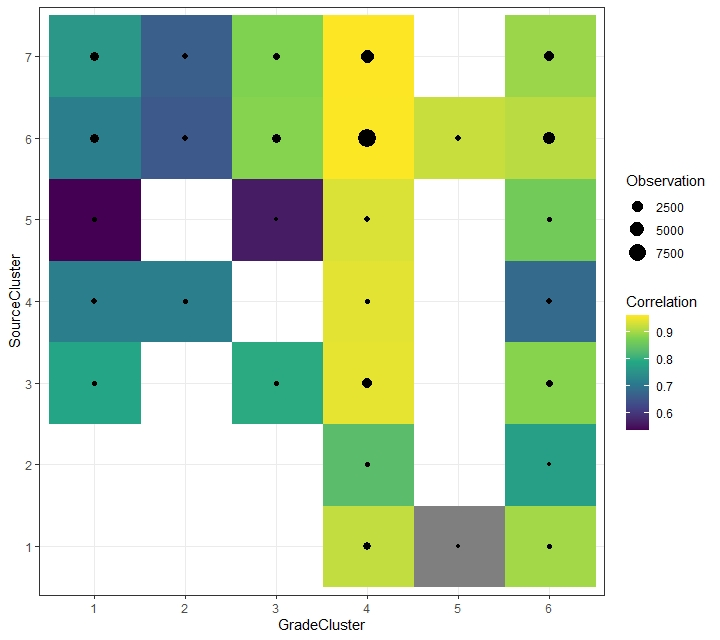
\includegraphics[width =0.5\textwidth]{figures/corrplot.jpeg}
    \caption{The correlation between Price and Valuation for different types of tea of varying grades and sources, with dots denoting the number of available observations.}
    \label{fig:corrplot}
\end{figure}

\subsection{Estimation of bid raising probability}

Since, each of the types of tea could have a different dropping patterns among bidders, we could use the usual Kaplan-Meier Product Moment Limit (KMPL) estimator~\cite{kleinbaum2010survival} to nonparametrically estimate the survival functions $S_i(t)$. Assuming we have $P_{(1)} < P_{(2)} < \dots P_{(k)}$ distinct selling prices without censoring, and at time $P_{(i)}$, $d_i$ bidders drops out of the remaining $n_i$ bidders, the KMPL estimate turns out to be given by the formula

$$
\widehat{S}(t) = \prod_{i : P_{(i)} < t} \left(  1 - \dfrac{d_i}{n_i} \right), \qquad \forall t \geq 0.
$$

\noindent Applying complementary log-log transformation to $S(t)$ and using delta method, one can show that an asymptotic $100(1-\alpha)\%$ confidence interval of $S(t)$ based on the KMPL estimate $\widehat{S}(t)$ can be obtained as 

\begin{equation*}
    \left( \exp\left[ -e^{\widehat{L}(t) + z_{1-\alpha/2}\widehat{\sigma}(t)} \right], \exp\left[ -e^{\widehat{L}(t) - z_{1-\alpha/2}\widehat{\sigma}(t)} \right] \right)
\end{equation*}

\noindent where 

\begin{align*}
    \widehat{L}(t) & = \log\left( -\log(\widehat{S}(t)) \right)\\
    \widehat{\sigma}(t) & = \dfrac{1}{\log(\widehat{S}(t))^2} \sum_{i : P_{(i)} < t} \dfrac{d_i}{n_i(n_i - d_i)}
\end{align*}

\noindent and $z_{1-\alpha/2}$ is the $(1 - \alpha/2)$-th quantile of the standard normal distribution. The KMPL estimate along with $95\%$ confidence intervals for the particular data has been computed and shown in Figure~\ref{fig:kmpl-est}. The effect of the sources on different gradeclusters are very different, for example, for tea type of grade cluster 3, the cluster of the source or origin of the tea does not affect the bidder's behavior much, while the behavior for grade cluster 4 has dependence with different origin or sources.

\begin{figure}[htb]
    \centering
    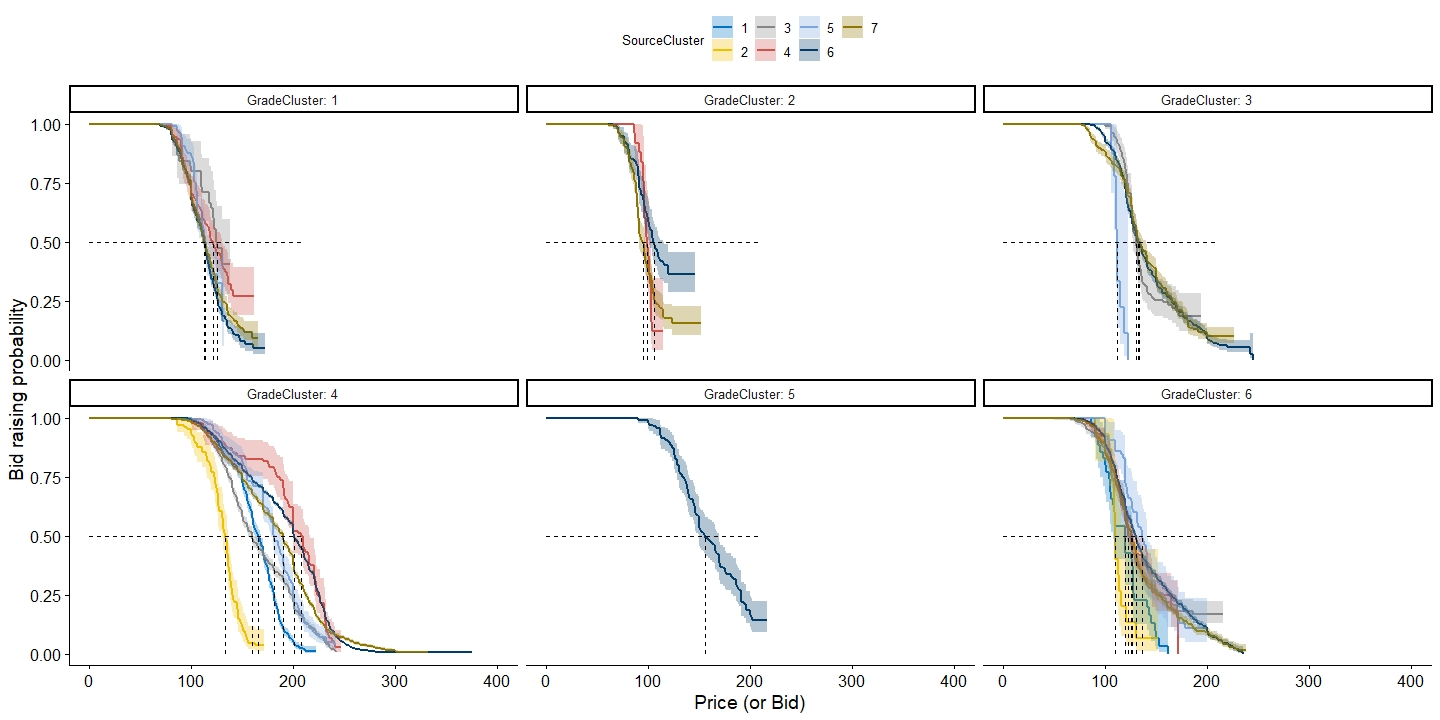
\includegraphics[width = \textwidth]{figures/kmpl-est.jpeg}
    \caption{KMPL estimate of Bid raising probability as a function of current price (or bid) for all source and grade clusters}
    \label{fig:kmpl-est}
\end{figure}

\subsection{Estimating objective valuation index}

Our secondary goal of obtaining a valuation index, which is representative of the quality of the tea packet can now be obtained from the estimated median of these survival curves. The median of the survival curve $S(t)$ is estimated as the median of $\widehat{S}(t)$, i.e. 

$$
\widehat{\text{Median}} = \widehat{S}^{-1}(1/2) = \inf_{t} \left\{ t: \widehat{S}(t) \geq 1/2 \right\}.
$$

\noindent This median of the survival curve theoretically represents the exact price at which exactly half of the available bidders are ready to purchase the item. If the initial valuation by the auction house is set lower than this price, then more bidders will be interested to make bids, hence the bidding will continue to grow up. On the other hand, if the initial valuation is set higher than this price, then less number of bidders will be interested, as a consequence, they will try to bargain at a lesser price than quoted. Therefore, this median represents an equilibrium price in the auction mechanism, hence could be used as a proxy of the subjective valuation provided by the auction house. For the combinations of Grade and Source where data is available, we have computed these estimates of the median, and they are summarized in Table~\ref{tbl:kmpl-median}. It shows that Grade 4 (consisting of D, CD, CHD etc.) is usually the most desirable grade of tea, hence is sown in all of the tea-making regions. On the flipside, Grade 2 (OCD, OD1 etc.) are usually sold at lesser price irrespective of the origin. 

\begin{table}[htb]
    \centering
    \begin{tabular}{c|cccccc}
        \toprule
        \textbf{Source} & \textbf{Grade 1} & \textbf{Grade 2} & \textbf{Grade 3} & \textbf{Grade 4} & \textbf{Grade 5} & \textbf{Grade 6}\\
        \midrule
        \textbf{Cluster 1} & NA & NA & NA & 166 & NA & 120 \\
        \textbf{Cluster 2} & NA & NA & NA & 133 & NA & 110 \\
        \textbf{Cluster 3} & 125 & NA & 130 & 160 & NA & 123\\
        \textbf{Cluster 4} & 121 & 99 & NA & 208 & NA & 106 \\
        \textbf{Cluster 5} & 114 & NA & 112 & 181 & NA & 136 \\
        \textbf{Cluster 6} & 113 & 106 & 132 & 201 & 156 & 130 \\
        \textbf{Cluster 7} & 114 & 95 & 133 & 190 & NA & 125 \\
        \bottomrule
    \end{tabular}
    \caption{Median bid for different types of tea of different source and grade clusters}
    \label{tbl:kmpl-median}
\end{table}

\subsection{Effect of subjective valuation on bid prices}

To understand the effect of the subjective valuation provided by the auction house ($V_i$) on the private valuation (or bid prices) by the bidders ($B_i$), we start with Cox's semi-parametric regression model. Under this model, we assume that $\lambda_i(t) = \lambda_0(t) \exp(\eta_i)$ where $\eta_i = \beta_1 \log(V_i) + \beta_2 \log(Q_i) + \sum_{j=1}^6 \beta_{3j} \ind{G_i = j} + \sum_{j=1}^7 \beta_{4j} \ind{O_i = j}$. Using the maximum partial likelihood approach, one can estimate the regression coefficients, and using Breslow's method, one can simultaneously estimate the baseline hazard $\lambda_0(t)$. With the same notation as before, if $\R(P_{(i)}-)$ denotes the risk set at price $P_{(i)}-$, then the estimate of cumulative baseline hazard function becomes 

\begin{equation}
\widehat{\Lambda_0}(t) = \sum_{i: P_{(i)} \leq t} \dfrac{d_i}{\sum_{k \in \R(P_{(i)}-)} \exp\left( \widehat{\eta}_k \right) }
\label{eqn:breslow-est}
\end{equation}

\noindent where $\widehat{\eta}_k$ is the $\eta_k$ with beta coefficients replaced by their estimates. We call this as \textbf{Model 1}. Based on the available data, we obtain

\begin{multline}
    \widehat{\eta}_i = -8.4291872 \log(V_i) + 0.3162530 \log(Q_i) + -0.0606649 \times \ind{G_i = 2} + \\
    0.1206609 \times \ind{G_i = 3} + \dots + 1.1791956\times\ind{O_i = 7}. 
    \label{eqn:model1-fit}
\end{multline}

\noindent The model showed that the log-valuation is a significant factor with a very low z-statistic $-175.626$ (i.e. the null hypothesis $\beta_{1} = 0$ would be rejected based on asymptotic score test). However, a negative coefficient for $\log(V_i)$ is doubtful, since it is expected that if the basic valuation increases, then a causal relationship would force the bidders to also increase their own private valuations. Turning to verify whether the proportional hazard assumptions are satisfied or not, we obtain the cox-snell residuals as $r_i = \widehat{\Lambda_0}(P_i)\exp(\widehat{\eta}_i)$, which under the null hypothesis of proportional hazard should be a censored sample from the exponential distribution of mean $1$. Therefore, the estimated cumulative hazard rate of the pseudo data $(r_i, \delta_i)$ should remain close to $y = x$ line. As seen from Figure~\ref{fig:kmpl-est}(a), this is clearly not the case for model 1, hence we can say that proportional hazard assumption is not satisfied.


\begin{figure}[htb]
    \centering
    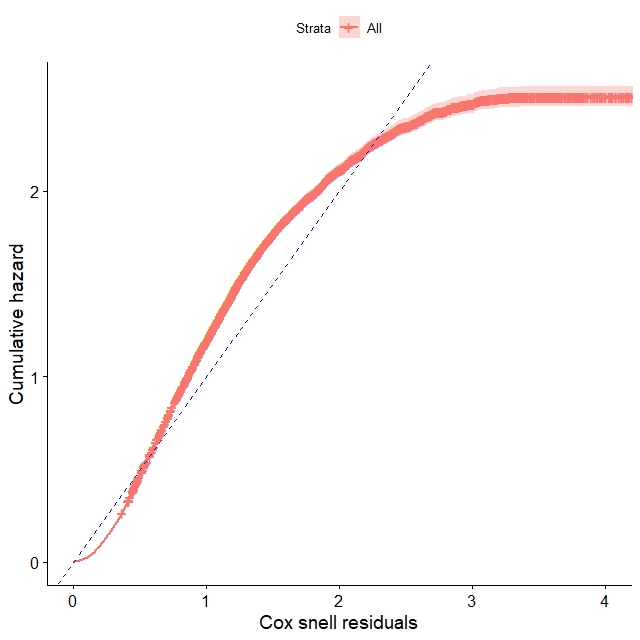
\includegraphics[width = 0.49\textwidth]{figures/coxph-1-resid.jpeg}
    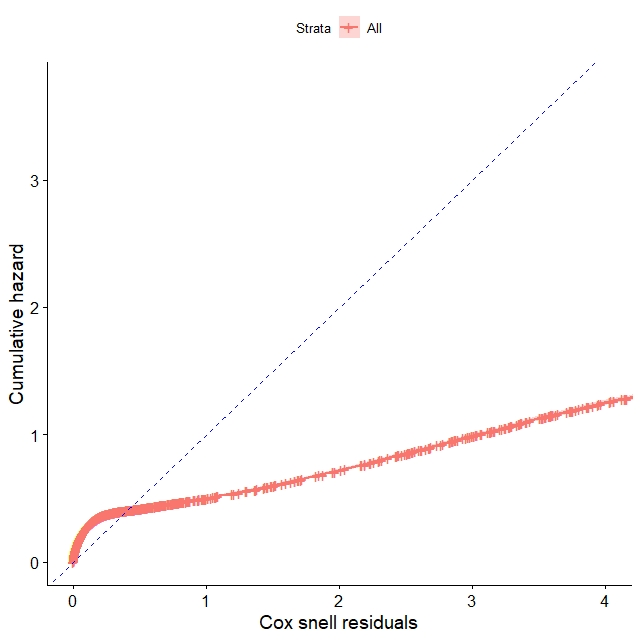
\includegraphics[width = 0.49\textwidth]{figures/coxph-2-resid.jpeg}
    \caption{(a) [Left] Cumulative hazard rates estimated from Cox-snell residuals of first model; (b) [Right] Cumulative hazard rates estimated from Cox-snell residuals of second model}
    \label{fig:coxsnell-resid}
\end{figure}

Since it is evident from Figure~\ref{fig:kmpl-est} that there are certain differences between the bid raising probability (or the survival function of $B_i$) between different types of tea of varying grades from varying sources, it seems that the proportionality assumption could be violated due to different baseline hazard in different strata. Therefore, we consider the categorical variables $(G_i, O_i)$ grouped together as a stratum and denote this by $St_i$, with $St_i$ taking values in $(1, 1), (1, 2) \dots (6, 7)$. Based on this stratum in effect, we consider a simple strata-based extension of Cox's regression model (\textbf{Model 2}) where the hazard function is expressed as

$$
\lambda_i(t) = \lambda_{0,St_i}(t) \exp(\xi_i)
$$

\noindent where $\xi_i = \beta_1 \log(V_i) + \beta_2 \log(Q_i)$ and $\lambda_{0, St_i}(t)$ is the baseline hazard corresponding to the strata $St_i$. In this case, since $\dfrac{\lambda_i(t)}{\lambda_j(t)} = \dfrac{\lambda_{0, St_i}(t)}{\lambda_{0, St_j}(t)} \exp(\xi_i - \xi_j)$, the proportionality assumption of Model 1 is violated. Again, the partial likelihood can be obtained by multiplying the partial likelihood from each stratum, and then one can obtain maximum partial likelihood estimators of the beta coefficients. In this way, we estimate the new Cox's equation as 

\begin{equation}
    \widehat{\xi}_i = -10.5525692 \log(V_i) + 0.3925898 \log(Q_i).
    \label{eqn:model2-fit}
\end{equation}

\noindent Again, the model shows log-valuation as a significant covariate in the Cox's regression, however, the coefficient of $\log(V_i)$ remaining negative is counter-intuitive. Therefore, we again see if proportional hazard assumptions are satisfied using the means of Cox-snell residuals. Similar to before, Breslow's estimator of cumulative baseline hazard for each stratum can be obtained through Eq.~\eqref{eqn:breslow-est} where the numerator will only consider $d_i$'s from the same strata but the denominator will remain the same as before. Here, the Cox-snell residuals are calculated as $r_i = \widehat{\Lambda}_{0, St_i}(P_i)\exp(\widehat{\xi}_i)$, and corresponding residuals and cumulative hazard based on $(r_i, \delta_i)$ is plotted in Figure~\ref{fig:coxsnell-resid}(b). Clearly, the residuals show even more deviation, suggesting that the Model 2 is not adequate for this data.

Next, we move towards a more general semi-parametric Accelerated Failure Time (AFT) model. Under this model, the private valuation (or bid prices) $B_i$ is assume to have a log linear representation

$$
Y_i = \log(B_i) = \alpha + \beta_1 \log(V_i) + \beta_2 \log(Q_i) + \sum_{j=1}^6 \beta_{3j} \ind{G_i = j} + \sum_{j=1}^7 \beta_{4j} \ind{O_i = j} + \sigma w
$$

\noindent where $w$ follows an unknown density function $f$. Such a representation is also in accordance to the log-normal distributional assumption mentioned in Dalal et. al.~\cite{dalal2020information}. Since no distributional assumption is made for $w$, this remains a semi-parametric approach. Miller~\cite{miller1976least} suggested a least squares approach to solve this problem where only the uncensored part of the data. Buckley and James~\cite{buckley1979linear} proposed an alternative to use the least squares on the whole data, but treat $Y_i^\ast$ as response variable where 

$$
Y_i^\ast = Y_i \delta_i + \mathbb{E}(Y_i \mid Y_i > \log(P_i)) (1 - \delta_i)
$$

\noindent where the conditional expectation is estimated using the KMPL estimate of the right censored data along with the most recent value of the estimate of the beta coefficients. Buckley and James suggested an iterative procedure that performs this estimate of $\mathbb{E}(Y_i \mid Y_i > \log(P_i))$ and then minimizes the least square to update the beta coefficients and iterate. Koul et al.~\cite{koul1981regression} extended that idea to include censoring distribution as well to compute the expectation. Miller~\cite{miller1982regression} and Kleinbaum and Klein~\cite{kleinbaum2010survival} provided an excellent review and comparison of these methods. For our purpose, we shall use Buckley and James estimator, computed via the following algorithm.

\begin{enumerate}
    \item Obtain some initial estimate $\widehat{\alpha}^{(0)}, \widehat{\beta}_1^{(0)} \dots \widehat{\beta}_{47}^{(0)}$.
    \item For $t = 0, 1, \dots$, repeat until convergence
    \begin{enumerate}
        \item Compute the residuals $e_i = \log(B_i) - \widehat{\alpha}^{(t)} - \widehat{\beta}_1^{(t)} - \dots \widehat{\beta}_{47}^{(t)} \ind{O_i = 7}$.
        \item Obtain KMPL estimate $\widehat{F}_{KM}(e)$ based on $(e_i, \delta)$. Let, it has a jump $w_i$ at $e_i$.
        \item Compute $B_i^\ast = B_i\delta_i + (1-\delta_i)\left[ \widehat{\alpha}^{(t)} - \widehat{\beta}_1^{(t)} - \dots \widehat{\beta}_{47}^{(t)} \ind{O_i = 7} + \dfrac{\sum_{j: e_j > e_i} e_j w_j }{\sum_{j: e_j > e_i} w_j} \right]$
        \item Update the estimates as
        $$
        \left( \widehat{\alpha}^{(t+1)}, \widehat{\beta}_1^{(t+1)} \dots \widehat{\beta}_{47}^{(t+1)} \right) = \arg\min \sum_{i=1}^n \left( Y_i^\ast - \widehat{\alpha}^{(t)} - \widehat{\beta}_1^{(t)} - \dots \widehat{\beta}_{47}^{(t)} \ind{O_i = 7} \right)^2
        $$
    \end{enumerate}
\end{enumerate}

\noindent An estimate of the standard error of the converged estimate $\widehat{\beta}^\ast = \left(\widehat{\alpha}^{\ast}, \widehat{\beta}_1^{\ast} \dots \widehat{\beta}_{47}^{\ast}\right)$ can be obtained as 

$$
\widehat{\text{Var}}(\widehat{\beta}^\ast) = \dfrac{1}{n_u - 14} \sum_u \left( Y_i -  \widehat{\alpha}^{\ast} - \widehat{\beta}_1^{\ast} - \dots \widehat{\beta}_{47}^{\ast} \ind{O_i = 7}\right)^2 (\boldsymbol{Z}^\intercal \boldsymbol{Z})^{-1}
$$

\noindent where $\boldsymbol{Z}$ is the design matrix, $n_u$ is the number of uncensored observations and $\sum_u$ denotes summation over only the uncensored observations. Based on the available data, the following regression equation is obtained

\begin{multline}
\widehat{Y}_i = \log(B_i) = -0.2541 +  1.1222 \log(V_i) - 0.0435\log(Q_i) +
0.0185 \times \ind{G_i = 2}\\
- 0.0447 \times \ind{G_i = 3} + -0.1393 \times \ind{G_i = 4} - 0.087 \times \ind{G_i = 5} - 0.0493\times \ind{G_i = 6}\\
- 0.0198\times \ind{O_i = 2} + 0.0229 \times \ind{O_i = 3} + 0.0726 \times \ind{O_i = 4}\\
+ 0.0143 \times \ind{O_i = 5} - 0.0103 \times \ind{O_i = 6} - 0.0016 \times \ind{O_i = 7}.
\end{multline}

\noindent We also found that the log-valuation and log-volume are significant factors here. Note that, here the coefficient of log-valuation is positive and coefficient of log-volume is slightly negative, which was expected. This means that when the auction house makes its valuation twice as large, then the private valuation $B_i$ increases $2.177$ times as large. The standard error of $\widehat{\beta}_1^\ast$ equal to as low as $0.0028$ also suggests that the estimate is quite reliable. On the other hand, if the quantity of the tea package increases, the usual demand supply equation motivates the bidders to decrease their private valuation (because they should be able to procure a lot with less per unit price and perishable nature ensures that auction house would try to sell even if the price is low). Finally, to check the model assumptions, similar to linear regression, we plot the fitted $Y_i$'s and the residuals in Figure~\ref{fig:bjmod-resid}. As seen from Figure~\ref{fig:bjmod-resid}, except few outlying observations, most of the residuals are randomly and densely packed near $0$, suggesting the goodness of the fitted AFT model.

\begin{figure}[htb]
    \centering
    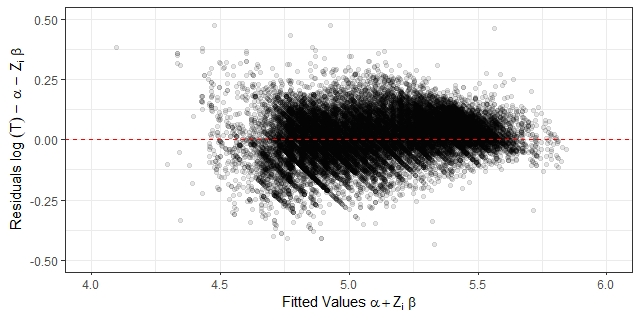
\includegraphics[width = \textwidth]{figures/bjmod-resid.jpeg}
    \caption{Fitted vs Residuals plot for Buckley James estimate of semi-parametric AFT model}
    \label{fig:bjmod-resid}
\end{figure}


\section{Conclusion}

The final model (i.e. the semi-parametric AFT model) suggested that it can correctly model the private valuations $B_i$ as a linear function of the log-transformed subjective valuation $V_i$ provided by the auction house, the volume of the package $Q_i$ and different grade and origin-specific characteristics of the tea. We found that the log-transformed subjective valuation $V_i$ is indeed a significant variable in determining the private valuations of the bidders. Therefore, the subjective valuation provided by the auction house is not necessarily just a quality measure of the tea package, but rather a carefully chosen price to increase their potential to sell. The bidders here are at a disadvantage, since the auction house has the ability to change the bidder's perception about a tea package, irrespective of its quality. To this end, the estimated survival curves or the bid raising probabilities could provide insights into the quality of the tea packages. The indices mentioned in Table~\ref{tbl:kmpl-median} should be able to help these bidders as a reference point to speculate whether the auctioneer is manipulating the price of some packages to their own profits, and take preventive measures. 

% bibliography
\bibliographystyle{unsrt}
\bibliography{references}
\end{document}
